\documentclass{beamer}
% \beamerdefaultoverlayspecification{<+->}
\usetheme{Madrid}

\title[Integer Factorisation]{Integer Factorisation Problem \& Modern Factoring Algorithms}
\author[VP and SB]{Vishisht Priyadarshi \& Sidharth Bankupalle\\[2ex] 
\includegraphics[scale=0.25]{iitg_logo.jpg}}
\institute[IITG]{Indian Institute of Technology Guwahati}
\centering
\date{May 2020}


\begin{document}
\maketitle
\begin{frame}{Content}
\begin{itemize}
    \item Introduction
    \item Factorisation Algorithms:
    \begin{itemize}
         \item Fermats's Factorisation Algorithm
         \item Pollards p-1 Algorithm
         \item Pollards Rho Algorithm
         \item Linear Sieve
    \end{itemize}
    \item Conclusion \& Future Prospects 
    \item References
\end{itemize}
\end{frame}

%%%%%%%%%%%%%%%%%%%%%%%%%%%%%%%%%%%%%%%%%%%%%%%%%%%%%%%%%%%%%%%%%%%%%%
\begin{frame}{Introduction}
\framesubtitle{Why do we need to care about Integer Factorisation}
\begin{itemize}
    \item The Integer Factorization problem is defined as follows:
    \textbf{Given a composite integer N, find a non-trivial factor e of N, i.e. find e such that e divides N.}
    \item When the numbers are sufficiently large, no efficient, non-quantum integer factorization algorithm is known.The most straightforward method of factoring is trial division, which, essentially, checks for every prime number $p$, such that $p \leq \sqrt{N}$ , if $p$ divides $N$. However, trial division may take more than $O\left( \sqrt {N}\right) $ bit operations, which makes it extremely inefficient for the numbers of interest.
    \item Currently there is no known algorithm for answering the question "Does integer N have a factor less than integer s?" in a number of steps that is $O\left( P\left( n\right) \right)$, where n is the number of digits in $N$, and $P\left(n\right)$ is a polynomial function. Moreover, no one has proved that such an algorithm exists, or does not exist
    
\end{itemize}
\end{frame}
\begin{frame}{Introduction (Contd.)}
   \begin{itemize}
       \item We are interested in factoring, because it is an example of an algorithmic problem on which there has been well-documented progress. Such examples should inform our expectations for algorithmic problems in general (including problems in AI).
        \item As well as their inherent interest and applicability to other areas of mathematics, advances in public key cryptography have lent algorithms for integer factorisation a lot of practical importance
       \item In this project, we aim to do an analysis of the modern Factoring Algorithms and their constraints.
\end{itemize}
\end{frame}
%%%%%%%%%%%%%%%%%%%%%%%%%%%%%%%%%%%%%%%%%%%%%%%%%%%%%%%%%%%%%%%%%%%%%%



%%%%%%%%%%%%%%%%%%%%%%%%%%%%%%%%%%%%%%%%%%%%%%%%%%%%%%%%%%%%%%%%%%%%%%
\begin{frame}{1. Fermat's Factorisation Method}
\framesubtitle{Algorithmic Perspective}
\begin{itemize}
    \item Consider $n$ to be an odd number(without loss of generality). If $n$ has a non-trivial factors, then $n$ can be written as $n = (x+y)(x-y)$ for some numbers $x$, $y$ $\in \mathbb{N}$ s.t. $x$, $y$ is not equal to $1$ and $n$.
    \item To implement this concept, we define a variable $a$ with initial value of $x^{2}-n$ where $x$ is initialised with a value of $\lfloor \sqrt {n}\rfloor $. Now we iterate over a loop until we found that $a$ is a perfect square. We update the value of $x$ over each iteration by adding odd numbers to it in a sequential way, starting from $2x+1$.
    \item That is, initially $a = x^{2}-n$, then after first iteration it becomes $\left( x+1\right) ^{2}-n$ since $\left( x+1\right) ^{2}=x^{2}+2x+1$. With each iteration, $a$ takes the values $\left( x+1\right) ^{2}-n$, $\left( x+2\right) ^{2}-n$ and so on until loop terminates. At the termination of the loop, we would have $a = x'^{2}-n$ where $a$ can be written as $a=y^{2}$. So, we have $n=x'^{2}-y^{2}$ and hence we have successfully factored $n$.
    
\end{itemize}
\end{frame}

\begin{frame}[fragile]{Algorithm}
\framesubtitle{Pseudo Code}
\begin{verbatim}
INPUT : Odd natural number, n
x <- Sqrt(n)
t <- 2x + 1
a <- x^2 - n
while(a is not a square of some k in N)
{
    a <- a + t
    t <- t + 2
}
x <- (t - 1)/2
y <- Sqrt(a)
return (x+y) and (x-y) as factors of n
\end{verbatim}
\end{frame}

\begin{frame}{Time Complexity}
    \begin{block}{Analysis}
    Let the odd composite number $n$ be written as $n=ab$. Then at the termination $a=x-y$ and $b=x+y$. Now to count the number of iterations, we can take help of $t$. Initially, $t$ will begin with $2x+1$. So, roughly $t$ can be considered to be $2\sqrt {n}$ and at the termination $t = 2x+1 = 1+a+b$.\break
Hence the number of iterations  = $\dfrac {1}{2}\left( 1+a+b-2\sqrt {n}\right) \\ \;\;\;\;\;\;\;\;\;\;\;\;\;\;\;\;\;\;\;\;\;\;\;\;\;\;\;\;\;\;\;\;\;\;\;\;\;\;\;\;\;\;\;\;\;\;\;\;= \dfrac {1}{2}\left( 1+a+\dfrac {n}{a}-2\sqrt {n}\right)\\ \;\;\;\;\;\;\;\;\;\;\;\;\;\;\;\;\;\;\;\;\;\;\;\;\;\;\;\;\;\;\;\;\;\;\;\;\;\;\;\;\;\;\;\;\;\;\;\;=
\dfrac {1}{2}\left( 1+\dfrac {\left( \sqrt {n}-a\right) ^{2}}{a}\right) $ 
\break\break
As it is evident that the algorithm performs poorly than Trial Division in some of the cases. It works well only when $a$ is very close to $\sqrt{
n}.$

    \end{block}
\end{frame}

\begin{frame}{Example}
\begin{block}{Factorising n = 527 }

\begin{table}[h!]
\centering
 \begin{tabular}{||c c c c||} 
 \hline
$ x & t\;=\;2x+1 & x^{2} & a\;=\;x^{2}-n $ \\ [0.5ex] 
 \hline\hline
 22 & 45 & 484 & -43 \\ 
 23 & 47 & 529 & 2 \\
 24 & 49 & 576 & 49 \\ [1ex] 
 \hline
 \end{tabular}
\end{table}
Hence $527=24^{2}-7^{2}=\left( 24-7\right) \left( 24+7\right)$
\end{block}
    
\end{frame}
%%%%%%%%%%%%%%%%%%%%%%%%%%%%%%%%%%%%%%%%%%%%%%%%%%%%%%%%%%%%%%%%%%%%%%



%%%%%%%%%%%%%%%%%%%%%%%%%%%%%%%%%%%%%%%%%%%%%%%%%%%%%%%%%%%%%%%%%%%%%%
\begin{frame}{2. Pollard’s p-1 Factorisation Algorithm}
\framesubtitle{Algorithmic Perspective}
\begin{itemize}
    \item Pollard's p - 1 Method is based on Fermat’s Little Theorem
    which says that $a^{p-1}\equiv 1\left( mod\;p\right) $ when $p$ is a prime which does not divide $a$.
    \item Therefore $a^{L}\equiv 1\left( mod\;p\right) $ for any multiple $L$ of $p-1$. If also $p | n$, then $p$ divides $gcd\left( a^{L}-1,n\right) $. Of course, we cannot compute $a^{L}$ mod $p$ because $p$ is an unknown prime factor of $n$.
    \item However, we can compute $a^{L}$ mod $n$. Pollard’s idea is to let $L$ have many divisors of the form $p − 1$ and thus try many potential prime factors $p$ of $n$ at once.
\end{itemize}
  
\end{frame}
\begin{frame}
\frametitle{Deeper Insights}
\begin{itemize}
    \item p is prime $\Rightarrow$ p - 1 is composite
    \item Let $p-1=a^{i_{1}}_{1}a^{i_{2}}_{2}\ldots a^{i_{k}}_{k}$ \quad \quad where $a_{1},a_{2},\ldots ,a_{k}$ are primes.
    \item Consider a number L s.t. $L\geq \max \left\{ a^{i_{1}}_{1}, a^{i_{2}}_{2}, \ldots , a^{i_{k}}_{k}\right\} $
    \break
    Now L! = L(L-1)(L-2)...1 must be divisible by p-1, since all prime powers of (p-1) exist in the terms of L! at least once.
    \item By Fermat's Little Theorem, for any arbitrary a \quad $a^{p-1}\equiv 1\left( mod \;p\right)$
    \break
    Now since $L!\equiv 0\left(mod\; p-1\right)  \Rightarrow   a^{L!}\equiv 1\left( mod \;p\right) \Rightarrow   a^{L!}-1\equiv 0\left( mod \;p\right) \Rightarrow $  p divides $a^{L!}-1$.\break
    $ \therefore \; \gcd \left( a^{L!}-1,n\right) =$ p or n
    \item We can compute this GCD. If it is not equal to n, we have found a prime factor of n, i.e., p. But if $\gcd \left( a^{L!}-1,n\right) = n  \Rightarrow$ n divides $a^{L!}-1 \Rightarrow$ q divides $a^{L!}-1 \Rightarrow a^{L!}\equiv 1\left( mod \;q\right)$.
    \break
    Now consider $L!=j\left( q-1\right) +k$ \quad , j, k $\in$ $\mathbb{Z}$  and k $\in$ [0, q-1]
    \break
    $\Rightarrow a^{L!}\equiv a^{k}\left( mod \;q\right) \Rightarrow \therefore a^{k}\equiv 1\left( mod \;q\right) $
\end{itemize}
\end{frame}

\begin{frame}
\frametitle{Deeper Insights (Contd.)}
\begin{itemize}
    \item \underline{Case (i) k = 0 :} We restart the process with a different random value of a.
    \break
    \underline{Case (ii) k $\neq$ 0 :} $a^{k}\equiv 1\left( mod \;q\right) $ holds true always until a is not divisible by q. But in no way, we can know before-hand if this is the case since p, q are unknown to us. So the best possible way is to restart the process with a random value of a.
    \item As we compute $a^{L!}$, and take gcd we have two cases:\break
    \underline{Case (i): } If d $>$ 1, we found the gcd and loop terminates.\break
    \underline{Case (ii): } If d = n, we go back and restart the algorithm with a new random value of a. It is guaranteed that we will run into some value of a which is multiple of one of the prime factors of n. In that case, gcd(a, n) $>$ 1. Say, p divides a, and p also divides $a^{L!}-1$
    $\Rightarrow \gcd \left( a^{L!}-1, \;n\right) = p$ . Hence the algorithm terminates.
    
\end{itemize}
\end{frame}


\begin{frame}[fragile]{Algorithm}
\framesubtitle{Pseudo Code}
\begin{verbatim}
INPUT : Natural number, n
a <- random()
for j <- 2 to BOUND(B)
{
    a <- a^j mod n
    d <- gcd(a-1, n)
    if(1 < d < n)
        return d
    else if (d = n)
        RESTART ALGORITHM WITH A NEW VALUE OF a
}
\end{verbatim}
\end{frame}


\begin{frame}{Time Complexity}
    \begin{block}{Key Points}
        \begin{itemize}
            \item There are $O\left( B\right)$ modular exponentiations, and each requiring $O\left(log B\right)$ multiplications.
            \item GCD can be computed in O(log n) time.
            \item $ \therefore$ Time Complexity $= O(B. log B. log n + log n) $
        \end{itemize}
    \end{block}
    
\end{frame}


\begin{frame}{Example}
\begin{block}{Factorising n = 10001 }
Let the random number be 2, i.e., $a$ = 2.
\begin{table}[h!]
\centering
 \begin{tabular}{||c c c||} 
 \hline
$ j & a\;=\; a^{j}\% n &  d\;=\;gcd\left(a-1,n\right) $ \\ [0.5ex] 
 \hline\hline
 1 & 2 & 1 \\ 
 2 & 4 & 1 \\
 3 & 64 & 1 \\
 4 & 5539 & 1 \\
 5 & 7746 & 1 \\
 6 & 1169 & 73 \\[1ex] 
 \hline
 \end{tabular}
\end{table}
Hence $10001 = 7*37 \therefore$ Prime factors of 10001 are 73 and 37.
\end{block}
    
\end{frame}
%%%%%%%%%%%%%%%%%%%%%%%%%%%%%%%%%%%%%%%%%%%%%%%%%%%%%%%%%%%%%%%%%%%%%%



%%%%%%%%%%%%%%%%%%%%%%%%%%%%%%%%%%%%%%%%%%%%%%%%%%%%%%%%%%%%%%%%%%%%%%
\begin{frame}{3. Pollard’s Rho Algorithm}
\framesubtitle{Algorithmic Perspective}
\begin{itemize}
    \item Pollard's rho algorithm iterates a simple polynomial map (which should not be a permutation polynomial) and produces a non-trivial divisor of n.
    \item The map generates a pseudo-random sequence of numbers (though the map generates random numbers, it has never been proved).
    \item Pollard's rho algorithm uses an iteration of the form:\quad \quad
    $x_{i+1}=f\left( x_{i}\right) mod \; n$ \quad , i $\neq$ 0   
    where $n$ is the number to be factored, $x_{0}$ is a random starting value and $f$ is a polynomial with integer coefficients.
    \item In practice, $f\left( x\right) = x^{2}+a$ is chosen ( a $\neq$ 0, -2 since they are fixed points for $f\left( x\right) $ ).
\end{itemize}
\end{frame}


\begin{frame}{Into the Algorithm}
The algorithm proceeds as follows :
\begin{block}{Steps}
\underline{STEP 1. :} Compute $d = gcd\left( x-x',n\right) ,\;\; x'=f\left( x\right) $\break\underline{STEP 2. :} If $1 < d < n$, d is a proper divisor of n. \break If d = 1, replace $x$ by $f\left( x\right)$, and $x'$ by $f\left(f\left( x'\right)\right)$ \break If d = n, algorithm has to be re-initialised, since we encountered a failure.
\end{block}
\begin{itemize}
    \item In short, we are looking for two distinct values $x_{i},x_{j}\in \mathbb{Z} _{n}$ s.t. $gcd\left( x_{i}-x_{j},n\right)  >1$. This is reasoned out by the fact that if $gcd\left( x_{i}-n_{j},n\right)  >1 \Rightarrow \; gcd\left( x_{i}-n_{j},n\right)$ is a factor of $n$, which is either $p$ or $q$.
    \item But whether we will get $gcd\left( x_{i}-n_{j},n\right)  >1$ and that too in reasonable number of steps is answered by the Birthday Paradox. In fact, Pollard's Rho Algorithm can be seen as a re-formulation of Birthday Paradox Problem, which we will discuss now:
\end{itemize}
\end{frame}


\begin{frame}{Analysis - Birthday Paradox and Pollard's Rho Algorithm}
    \begin{block}{}
        Say we pick $k$ numbers $x_{1},x_{2},\ldots ,x_{k}$ uniformly at random in  $\mathbb{Z} _{n}$. Suppose that these $k$ numbers are distinct. Now let's say that there exists some $1\neq i < j \neq k$ s.t. $x_{i}=x_{j}\left( mod\:p\right) $. Then $p\;|\;x_{i}-x_{j}$, and since $p\;|\;n$ also , we have $p\;|\;gcd\left( x_{i}-x_{j},n\right)$.
    \end{block}
    \begin{block}{}
         Moreover since $x_{i}, x_{j} \in \mathbb{Z}_{n}$ and they are distinct $\Rightarrow gcd\left( x_{i}-x_{j},n\right) < n \Rightarrow \; \therefore gcd\left( x_{i}-x_{j},n\right)$ provides a non-trivial factor of $n$.
    \end{block}
    \begin{block}{}
        But we need to find an upper-bound on size of k such that it is guaranteed that if we compute $gcd\left( x_{i}-x_{j},n\right)$ for all pairs of $1 \leq i < j \leq k$, we find a non-trivial factor.
    \end{block}
\end{frame}



\begin{frame}{Analysis (Contd.)}
\begin{itemize}
    \item Now, 
    \begin{equation}
      \label{q-def}
     x_{i}\equiv x_{j}\left( mod \; p\right)
    \end{equation}
    \item The probability that equation~\eqref{q-def} does not hold, i.e., $\left( x_{1},x_{2},\ldots ,x_{k}\right) mod \; p $ are all different is:
    \begin{equation}
    \mathbb{P} = \left( 1-\dfrac {1}{n}\right) \left( 1-\dfrac {2}{n}\right) \ldots \left( 1-\dfrac {k-1}{n}\right) 
    \sim e^{\dfrac {-k^{2}}{2n}}
    \end{equation}
    \item Since $p \leq \sqrt{n}$, $k = n^{\dfrac {1}{4}}$ is suitable since it gives a higher probability that (1) holds.\\
    Now we use the pseudo-random generator function to generate the k numbers in sequence and search for the pair i, j s.t. $i < j$ and $x_{i} \equiv x_{j} \left( mod \; p \right). $ But checking all the $\begin{pmatrix}
    k \\ 2 \end{pmatrix}$ pairs will result in a lot of GCD computations, thereby resulting in time complexity which is of the order $\sqrt {n}$. \break \break
    \item An optimisation that we can make here is to reduce the number of GCD computations by using Floyd's Cycle Detection Algorithm. Using this
    we will be able to deduce that there exists a pair $i < j < C_{o}\sqrt{p}$ \quad ($C_{o}$ is a constant) s.t. $x_{i} \equiv x_{j} \left( mod \; p \right)$ (based on empirical calculations). So our algorithm finds out the factor of n in $O\left( n^{1/4}\right)$ time.
\end{itemize}
\end{frame}



\begin{frame}{Analysis (Contd.)}
\begin{block}{Detecting Cycle}
    An optimisation that we can make here is to reduce the number of GCD computations by using Floyd's Cycle Detection Algorithm. Using this
    we will be able to deduce that there exists a pair $i < j < C_{o}\sqrt{p}$ \quad ($C_{o}$ is a constant) s.t. $x_{i} \equiv x_{j} \left( mod \; p \right)$ (based on empirical calculations). So our algorithm finds out the factor of n in $O\left( n^{1/4}\right)$ time.
    \end{block}
\end{frame}



\begin{frame}[fragile]{Algorithm}
\framesubtitle{Pseudo Code}
\begin{verbatim}
INITIALISE POLYNOMIAL MAP f
x  <- x_o
x' <- f(x) (mod n)
p  <- gcd(x - x', n)
while(p = 1)
{
    x  <- x_i
    x' <- x_2i
    x  <- f(x) (mod n)
    x' <- f(x')(mod n) { Executed Twice }
    p  <- gcd(x - x', n)
}
if(p = n)
    return "n is prime"
else
    return p
\end{verbatim}
\end{frame}


\begin{frame}{Time Complexity}
    \begin{block}{Key Point}
        The Pollard's Rho algorithm is able to find a factor $p$ of $n$ with an expected number of $\Theta \left( \sqrt {p}\right) $ of arithmetic operations, that is, about an order of $\Theta \left( \sqrt {n}\right)$.
    \end{block}
\end{frame}


\begin{frame}{Example}
    \begin{itemize}
        \item Let $f\left( x\right) =x^{2}+1$ be the sequence generator (our polynomial map).
        \item Factorise $n$ = 455459; Let $x_{o}$ = 2
    \end{itemize}
    \begin{block}{Computation}
        \begin{table}[h!]
        \centering
             \begin{tabular}{||c c c||} 
                 \hline
                $ x = f(x)& x'\;=\; f(f(x))\% n &  p\;=\;gcd\left(x-x',n\right) $ \\ [0.5ex] 
                 \hline\hline
                 5 & 26 & 1 \\ 
                 26 & 2871 & 1 \\
                 677 & 179685 & 1 \\
                 2871 & 155260 & 1 \\
                 44380 & 416250 & 1 \\
                 179685 & 43670 & 1 \\
                 121634 & 164403 & 1 \\
                 155260 & 247944 & 1 \\
                 44567 & 68343 & 743 \\[1ex] 
                 \hline
             \end{tabular}
        \end{table}
        $\therefore n = 613 * 743$
    \end{block}
    
    \begin{itemize}
        \item $\therefore n = 613 * 743$
    \end{itemize}
\end{frame}
%%%%%%%%%%%%%%%%%%%%%%%%%%%%%%%%%%%%%%%%%%%%%%%%%%%%%%%%%%%%%%%%%%%%%%



%%%%%%%%%%%%%%%%%%%%%%%%%%%%%%%%%%%%%%%%%%%%%%%%%%%%%%%%%%%%%%%%%%%%%%
\begin{frame}{4. Linear Sieve}
\framesubtitle{Algorithmic Perspective}
    \begin{itemize}
        \item The sieve of Eratosthenes is probably the simplest way to pick out all the primes in a given range from $2$ to $n$ but it has time complexity $O\left( n\log \log n\right) $.
        \item The Linear Sieve algorithm is similar to the classic Sieve of Eratosthenes but has linear complexity.
        \item Our goal is to calculate minimum prime factor $lp\left[ i\right] $ for every number $i$ in the segment $\left[ 2,n\right]$.
        \item We need to store the list of all the found prime numbers - let's call it $pr\left[ \right] $.
    \end{itemize}
\end{frame}


\begin{frame}{Algorithm}
    \begin{itemize}
        \item We'll initialize the values $lp\left[ i\right]$ with zeros, which means that we assume all numbers are prime. During the algorithm execution this array will be filled gradually. Now we'll go through the numbers from $2$ to $n$. We have two cases for the current number $i$:
    \end{itemize}
        
    \begin{block}{Case 1 : $lp\left[ i\right]=0$}
        This means that i is prime, i.e. we haven't found any smaller factors for it. Hence, we assign $lp\left[ i\right]=i$ and add $i$ to the end of the list $pr\left[ \right] $.
    \end{block}
    \begin{block}{Case 2 : $lp\left[ i\right]\neq 0$}
        This means that $i$ is composite, and its minimum prime factor is $lp\left[ i\right]$.
    \end{block}
    
    \begin{itemize}
        \item Let's consider numbers $x_{j}=i\cdot p_{j}$, where $ p_{j}$ are all prime numbers less than or equal to $lp\left[ i\right]$ (this is why we need to store the list of all prime numbers).\break
        We'll set a new value $lp\left[ x_{j}\right] =p_{j}$ for all numbers of this form.
    \end{itemize}
\end{frame}

\begin{frame}[fragile]{Algorithm}
\framesubtitle{Pseudo Code}
\begin{verbatim}
Enter a natural number n
Initialise array lp[n]
Initialise list pr
for i <- 2 to n
{
    if(lp[i] = 0)
    {
        lp[i] <- i
        push back i to pr
    }
    for j <- 1 to size(pr)
        if(pr[j] <= lp[i] AND (i*pr[j]) <= n)
            lp[i*pr[j]] = pr[j]
}
return lp[]

\end{verbatim}
\end{frame}


\begin{frame}{Time \& Space Complexity}
    \begin{block}{Key Points}
    \begin{itemize}
        \item Its time complexity is $O\left( n\right) $ which is slightly better than $O\left( n\log \log n\right) $.
        \item Considering the memory requirements of this algorithm - an array $lp\left[ \right] $ of length n, and an array of $pr\left[ \right] $ of length $\dfrac {n}{\ln n}$, this algorithm requires 32 times the memory needed for the classic sieve.
        \item However,this algorithm calculates an array $lp\left[ \right] $, which allows us to find factorization of any number in the segment $\left[ 2;n\right] $ in the time of the size order of this factorization.
    \end{itemize}
    \end{block}
    
\end{frame}


\begin{frame}{Example}
    \begin{itemize}
        \item Let n = 10 
        \item Initialise lp[2:10] to 0, and an empty list pr
        \begin{block}{Computation}
            \begin{table}[h!]
            \centering
                 \begin{tabular}{||c c c c c||} 
                     \hline
                    $ i & lp[](Outer Loop) & pr & j & lp[](Inner Loop) $ \\ [0.5ex] 
                     \hline\hline
                     2 & lp[2] = 2 & 2 & 1 & lp[4] = 2 \\
                     3 & lp[3] = 3 & 2, 3 & 1 & lp[6] = 2 \\
                     3 & - & 2, 3 & 2 & lp[9] = 3 \\
                     4 & - & 2, 3 & 1 & lp[8] = 2 \\
                     5 & lp[5] = 5 & 2, 3, 5 & - & - \\
                     6 & - & 2, 3, 5 & - & - \\
                     7 & lp[7] = 7 & 2, 3, 5, 7 & - & - \\
                     8 & - & 2, 3, 5, 7 & - & - \\
                     9 & - & 2, 3, 5, 7 & - & - \\
                     10 & - & 2, 3, 5, 7 & - & - \\[1ex]
                     \hline
                 \end{tabular}
            \end{table}
        \end{block}
        
    \end{itemize}
\end{frame}
%%%%%%%%%%%%%%%%%%%%%%%%%%%%%%%%%%%%%%%%%%%%%%%%%%%%%%%%%%%%%%%%%%%%%%



%%%%%%%%%%%%%%%%%%%%%%%%%%%%%%%%%%%%%%%%%%%%%%%%%%%%%%%%%%%%%%%%%%%%%%
\begin{frame}{Conclusion}
\begin{itemize}
    \item We are interested in factoring, because it is an example of an algorithmic problem on which there has been well-documented progress. As well as their inherent interest and applicability to other areas of mathematics, advances in public key cryptography have lent algorithms for integer factorisation a lot of practical importance.
    \item The general number field sieve (GNFS) is the most efficient classical algorithm known for factoring integers larger than $10^{100}$. It is a randomized algorithm and heuristically, we get an expected complexity of $O\Big(e^{\sqrt{\frac{64}{9}}(\log N)^{\frac 13}(\log\log N)^{\frac 23}}\Big)$.
    \item GNFS has been to able factor numbers up to 576 bits long. However, it seems quite improbable that a PC-based implementation of the algorithm can do much better. That is why, other, non-algorithmic methods, have been proposed to improve the efficiency of the existing algorithms.
    \item Some of these includes ideas of Distributed Computing, use of special hardwares(like Sieve Devices) and use of Quantum Computers (Shor's Algorithm). 
\end{itemize}
    
\end{frame}


\begin{frame}{Special Purpose Integer Factorisation Algorithms}
 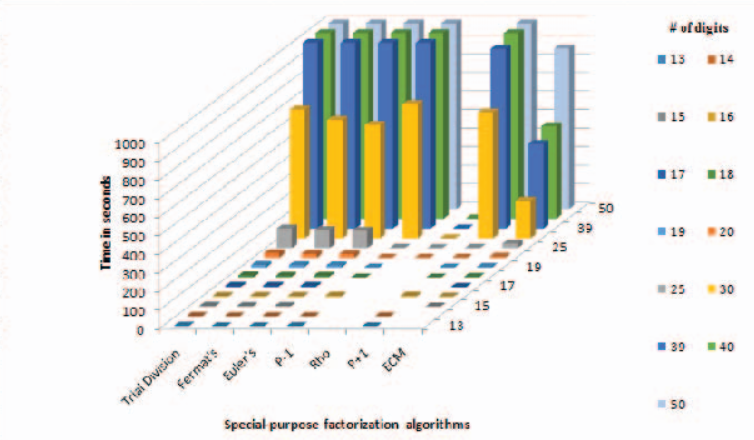
\includegraphics[height=6.8cm]{Comparison-2.png}
\centering   
\end{frame}


\begin{frame}{General Purpose Integer Factorisation Algorithms}
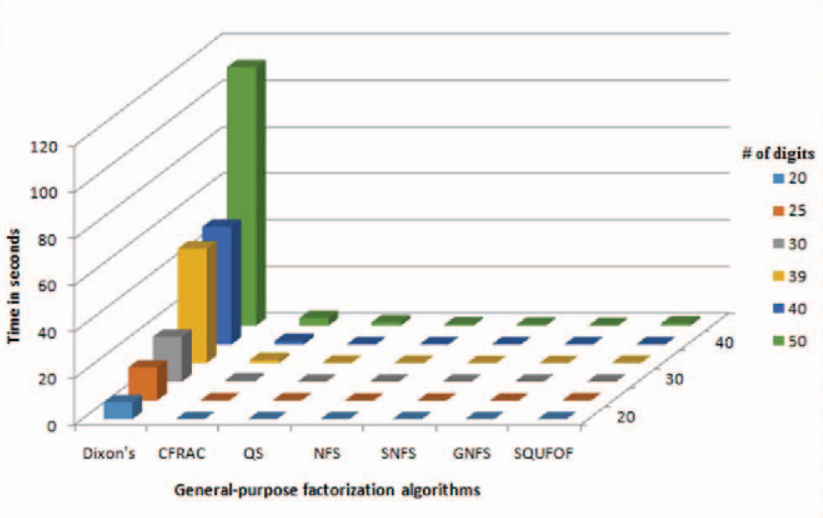
\includegraphics[height=6.8cm]{Comparison-1.png}
\centering
\end{frame}
%%%%%%%%%%%%%%%%%%%%%%%%%%%%%%%%%%%%%%%%%%%%%%%%%%%%%%%%%%%%%%%%%%%%%%



%%%%%%%%%%%%%%%%%%%%%%%%%%%%%%%%%%%%%%%%%%%%%%%%%%%%%%%%%%%%%%%%%%%%%%
\begin{frame}{References}
    \begin{enumerate}
        \item Arjen K. Lenstra, \emph{General purpose integer factoring}
        \item Kostas Bimpikis and Ragesh Jaiswal, \emph{Modern Factoring Algorithms}
        \item Richard P. Brent, \emph{An improved Monte Carlo Factorization Algorithm}, $\left( 1980\right)$ 
        \item Peter L. Montgomery, \emph{Speeding the Pollard and Elliptic Curve Methods of Factorization}, \emph{Mathematics of Computation,} Volume 48, Issue 177 (Jan.,1987), 243-264
        \item Eric Bach ,\emph{Toward a Theory of Pollard's Rho Method}, $\left( 1991\right)$
        \item David Gries \& Jayadev Misra, \emph{A Linear Sieve
    Algorithm for Finding Prime Numbers }
        \item Anne-Sophie Charest, \emph{Pollard’s p-1 and Lenstra’s factoring
        algorithms}, $\left( 2005\right)$
        \item Sounak Gupta and Goutam Paul, \emph{Revisiting Fermat’s Factorization
        for the RSA Modulus} $\left( 2009\right)$
        \item Robert Erra and Christophe Grenier, \emph{The Fermat factorization method revisited}, $\left( 3oth June 2009\right)$
        \item Cristina-Loredana Duta et al., \emph{Framework for evaluation and comparison of integer factorization algorithms}, 2016 SAI Computing Conference $\left( 2016\right)$
    \end{enumerate}      
\end{frame}
%%%%%%%%%%%%%%%%%%%%%%%%%%%%%%%%%%%%%%%%%%%%%%%%%%%%%%%%%%%%%%%%%%%%%%

\begin{frame}
\huge{\centerline{Thank You}}
\end{frame}

\end{document}
